\documentclass[10pt]{article}
\usepackage[polish]{babel}
\usepackage[utf8]{inputenc}
\usepackage[T1]{fontenc}
\usepackage{amsmath}
\usepackage{amsfonts}
\usepackage{amssymb}
\usepackage[version=4]{mhchem}
\usepackage{stmaryrd}
\usepackage{graphicx}
\usepackage[export]{adjustbox}
\graphicspath{ {./images/} }
\usepackage{hyperref}
\hypersetup{colorlinks=true, linkcolor=blue, filecolor=magenta, urlcolor=cyan,}
\urlstyle{same}

\title{PRACA KONTROLNA nr 1 - POZIOM PODSTAWOWY }

\author{}
\date{}


\begin{document}
\maketitle
\begin{enumerate}
  \item Z miast A i B odległych o 700 km o tej samej godzinie wyruszają naprzeciw siebie (po dwu równoległych torach) dwa pociągi. Pociąg pospieszny, który wyjeżdża z B, jedzie z prędkością o $35 \mathrm{~km} / \mathrm{h}$ większą niż wyjeżdżający z A pociąg osobowy i przyjeżdża do A godzinę wcześniej niż pociąg osobowy osiąga B. Z jakimi prędkościami poruszają się pociągi i w jakiej odległości od A się minęły.
  \item Wyznaczyć dziedziny funkcji $f(x)=\sqrt{\frac{|x-1|-4}{x+2}}$ oraz $g(x)=f(x+1)$ i $h(x)=f(|x|)$.
  \item Liczby
\end{enumerate}

$$
p=\frac{(\sqrt[3]{54}-2)(9 \sqrt[3]{4}+6 \sqrt[3]{2}+4)-(2-\sqrt{3})^{3}}{\sqrt{3}+(1+\sqrt{3})^{2}} \quad \text { i } q=\frac{64^{\frac{1}{3}} \sqrt{8}+8^{\frac{1}{3}} \sqrt{64}}{\sqrt[3]{64 \sqrt{8}}(1+\sqrt{2})}
$$

są miejscami zerowym trójmianu kwadratowego $f(x)=x^{2}+a x+b$. Znaleźć najmniejszą i największą wartość $f(x)$ na przedziale $[0,5]$.\\
4. Niech $f(x)=x^{2}$. Narysować wykres funkcji $g(x)=|f(x-1)-4|$ i określić liczbę rozwiązań równania $g(x)=m$ w zależności o parametru $m$.\\
5. Wykresy funkcji $f(x)=\frac{m-1}{m+2} x+1$ i $g(x)=\frac{m+2}{m-3} x+1$ są prostymi prostopadłymi. Obliczyć pole trójkata ograniczonego wykresami tych funkcji i osią $O x$. Podać równanie okręgu opisanego na tym trójkącie. Sporządzić rysunek.\\
6. W kwadrat $A B C D$ wpisano kwadrat $E F G H$, który zajmuje 3/4 jego powierzchni. Wyznaczyć wartości wszystkich funkcji trygonometrycznych mniejszego z kątów trójkąta EBF.\\
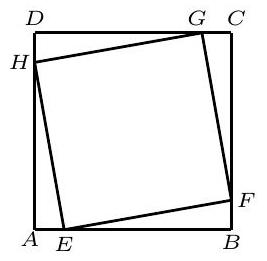
\includegraphics[max width=\textwidth, center]{2024_11_16_77c2ef888396535263bbg-1}

\section*{PRACA KONTROLNA nr 1 - POZIOM ROZSZERZONY}
\begin{enumerate}
  \item Statek wyrusza (z biegiem rzeki) z przystani A do odległej o 140 km przystani B. Po upływie 1 godziny wyrusza za nim łódź motorowa, dopędza statek w połowie drogi, po czym wraca do przystani A w tym samym momencie, w którym statek przybija do przystani B. Wyznaczyć prędkość statku i prędkość łodzi w wodzie stojącej, wiedząc, że prędkość nurtu rzeki wynosi $4 \mathrm{~km} /$ godz.
  \item Narysować wykres funkcji $f(x)=\min \left\{x^{3}, \frac{1}{x}\right\}$ i wyznaczyć jej dziedzinę oraz zbiór wartości. Podać wzór funkcji $h(x)$, której wykres jest symetryczny do wykresu $f(x)$ względem punktu $(0,0)$. Określić liczbę rozwiązań równania $f(x)=m$ w zależności o parametru $m$.
  \item Dla jakich wartości rzeczywistego parametru $p$ równanie $(p-1) x^{2}-(p+1) x-1=0$ ma dwa pierwiastki tego samego znaku odległe co najwyżej o 1?
  \item Wykresy funkcji $f(x)=(m-1) x+1$ i $g(x)=\frac{m}{m-1} x+b$ są prostymi prostopadłymi, a pole trójkata ograniczonego wykresami tych funkcji i osią $O x$ jest równe polu trójkąta ograniczonego tymi wykresami i osią $O y$. Wyznaczyć wzory funkcji $f$ i $g$ i obliczyć pole rozważanych trójkątów. Sporządzić rysunek.
  \item Obliczyć wartości
\end{enumerate}

$$
p=\sqrt{19-8 \sqrt{3}}-\sqrt[3]{26-15 \sqrt{3}} \quad \text { i } \quad q=\frac{14 \log _{9} \frac{1}{2}-\log _{\sqrt[3]{3}} \frac{1}{4}}{\log _{9} 8+\log _{\sqrt{3}} \frac{1}{2}}
$$

Następnie wyznaczyć wzór i narysować wykres funkcji $f(x)=\frac{a x+b}{c x+d}$, wiedząc, że jest on symetryczny względem punktu $(p, q)$ i przechodzi przez punkt $(0,0)$.\\
6. Punkt $D$ dzieli bok $A B$ trójkąta równobocznego $A B C$ w stosunku 2:1. Wyznaczyć stosunek długości promienia okręgu wpisanego w trójkąt $A D C$ do długości promienia okręgu wpisanego w trójkąt $D B C$.

Rozwiązania (rękopis) zadań z wybranego poziomu prosimy nadsyłać do 28 września 2016r. na adres:

Wydział Matematyki\\
Politechnika Wrocławska\\
Wybrzeże Wyspiańskiego 27\\
50-370 WROCEAW.\\
Na kopercie prosimy koniecznie zaznaczyć wybrany poziom! (np. poziom podstawowy lub rozszerzony). Do rozwiązań należy dołączyć zaadresowaną do siebie kopertę zwrotną z naklejonym znaczkiem, odpowiednim do wagi listu. Prace niespełniające podanych warunków nie będą poprawiane ani odsyłane.

Adres internetowy Kursu: \href{http://www.im.pwr.edu.pl/kurs}{http://www.im.pwr.edu.pl/kurs}


\end{document}